\documentclass{jarticle}
\usepackage{SICE-CCS}
\usepackage[dvipdfmx]{graphicx}
\usepackage{subfigure}
\usepackage{amsmath}
\usepackage{amssymb}
\usepackage{stmaryrd}
\usepackage{amsfonts}
\usepackage{bm}
\usepackage{ccaption}
\usepackage{comment}

\usepackage{multirow}
\pagestyle{empty}

\begin{document}

\title{ちびチャレ2019成果報告}
\author{B班(深津蓮,島田航太,吉内航,土屋一朗)}
\date{2019年4月26日}
\maketitle

\section{緒言}
近年,自動運転車を中心とした自律移動ロボットの研究開発が盛んに行われている.これらのロボットが自律移動を行うためには,自己位置推定,大域経路計画,局所経路計画,環境認識などが非常に重要である.これらの技術はROSのnavigation stack\cite{ns}などのオープンソースソフトウェアを用いて容易に実装可能である.しかし,今回はオープンソースソフトウェアを使用せずにそれらの技術を実装することで,コーティング技術と共に基礎的なロボット技術を学ぶことを目的とする.ハードウェアとしては,iRobot社のRoomba\cite{roomba}と北陽電機社の2D-LiDARのUTM-30LX\cite{lrf},Raspberry PI財団のRaspberry PI Model B+\cite{raspi},logicool社のC270 HD WEBCAM\cite{webcam},ノートPCを用いる.今回は,障害物を避け,白線を検知したら一回転し,最終的に明治大学生田キャンパス第二校舎D館1階を1周することを課題とする.

\section{提案手法}
本章では,提案システムにおける自己位置推定,大域経路計画,局所経路計画,白線検知について述べる.自己位置推定及び大域経路計画で用いる地図については,オープンソースソフトウェアのgmapping\cite{gmapping}を用いて作成した.システム図をFig.\ref{fig:system}に示す.

\subsection{自己位置推定}
自己位置推定にはAugmented Monte Carlo Localization(AMCL)\cite{localization}を用いた.観測モデルのノイズとして,正しい計測時の局所的な計測ノイズ,事前地図の中に存在しない物体による計測ノイズ,レーザがガラスなどを透過したことによる計測ノイズ,ランダムに発生する計測ノイズの4種類の観測ノイズを想定した.これらを導入することで,本試験中に想定されるノイズに対して強い尤度計算ができるようにした.また,Eq.\ref{eq:localization}に示す全パーティクルの平均に比例する確率$p$でランダムパーティクルを追加し,位置推定誤差からの復帰ができるようにした.ここで,$\omega_{fast}$,$\omega_{slow}$はそれぞれ尤度の短期および長期の平均値である.これと併用してパーティクルのxy座標およびyaw角の分散が閾値以下になると,最新の推定位置の周りにパーティクルを初期化することにより,システムのロバスト性を高めた.

\begin{equation}
	p = max(0.0 , 1-\frac{\omega_{fast}}{\omega_{slow}})
	\label{eq:localization}
\end{equation}


\begin{figure}
	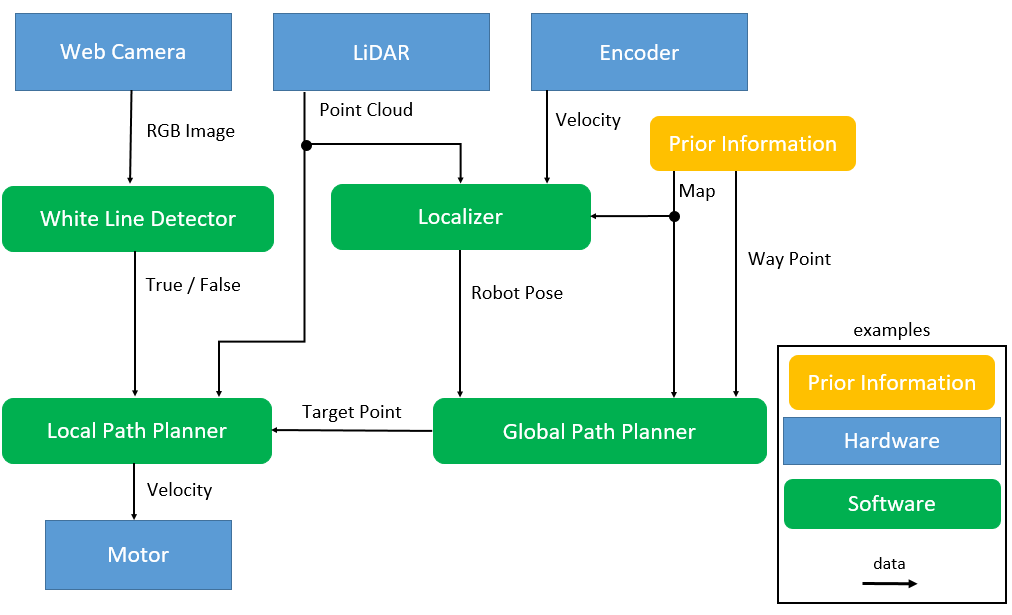
\includegraphics[width=8.5cm]{./picture/system.png}
	\caption{システム図}
	\label{fig:system}
\end{figure}

\begin{figure}
	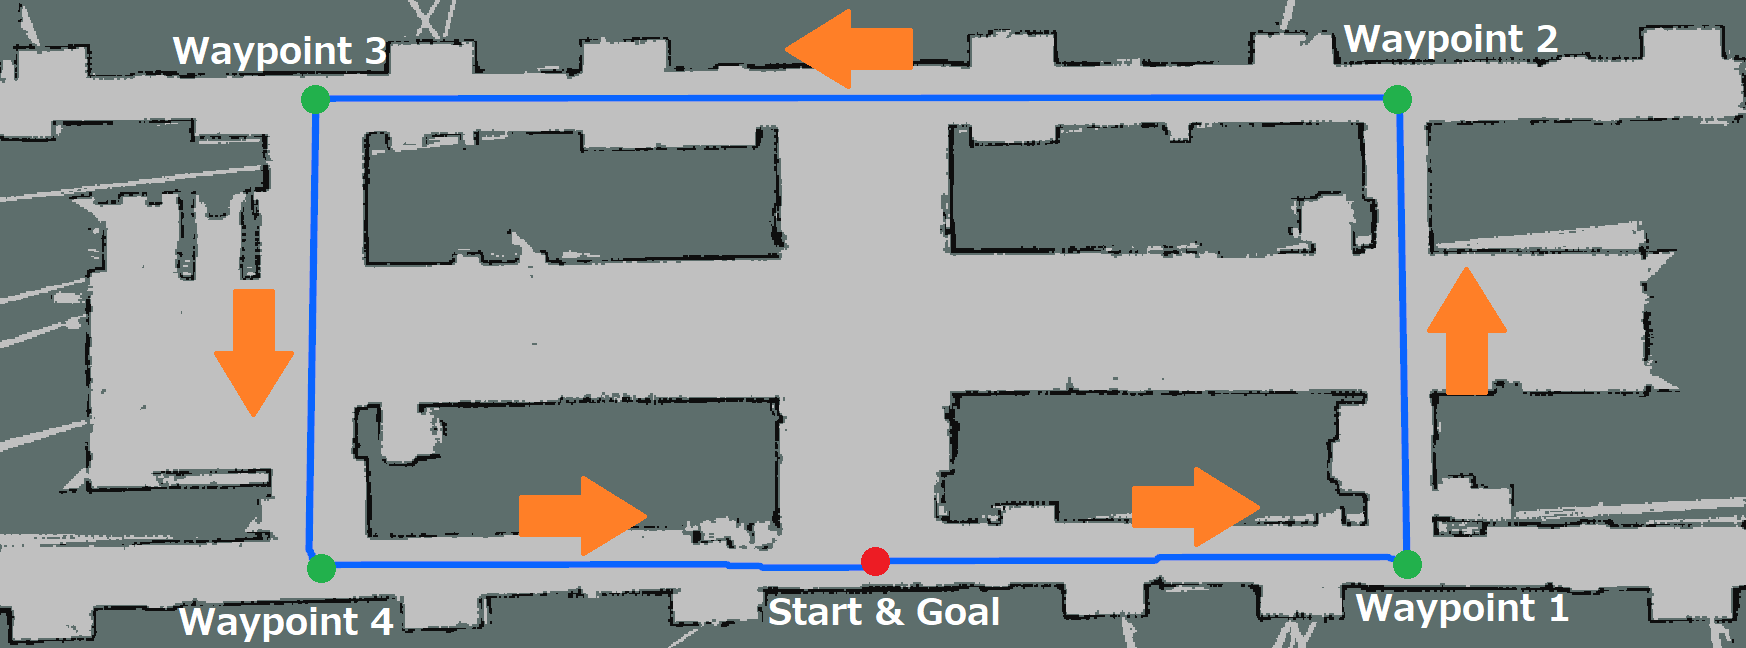
\includegraphics[width=8.5cm]{./picture/global_path.png}
	\caption{大域経路}
	\label{fig:globalpath}
\end{figure}


\subsection{大域経路計画}
大域経路計画には,A*アルゴリズムを用いた.この経路計画において,地図はセルの集合として扱う.開始地点のセルから経路探索を始め,そのセルに到達するための最小コスト$g$と目標地点からの距離のヒューリスティック値$h$の和が最小のセルを選択して探索を進めていく.これにより,全経路を探索することなく最短経路を導き出すことができる.しかし,このままでは経路が壁に沿って壁と接してしまう.これを改善するために,h値とg値に壁からの距離に基づくw値を足した値をfとすることで壁から少し離れた経路を選択するようにした.最終的なfの値をEq.\ref{eq:globalpath}に示す.
\begin{equation}
	f = g + h + w
	\label{eq:globalpath}
\end{equation}

Fig.\ref{fig:globalpath}に導き出した経路を示した.この経路は,機体の位置から次の目標地点を定めるときに用いた.自己位置から一番近い大域経路の点を調べ,その点から経路上で1.5m先の点を目標地点と定めるという方法で行った.


\subsection{局所経路計画}                                                  
局所経路計画にはDynamic Window Approachを用いる.
Dynamic Window内の速度$v$, 角速度$\omega$ をサンプリングし経路を予測する.
そして,コストを計算し,コストが最少となる速度$v$ ,角速度$\omega$ を出力値とする.ここで,コスト計算には予測経路と障害物までの最短距離である$obs(v,\omega)$,最終予測位置から目標地点までの距離である$dis(v,\omega)$,目標位置に対する機体の向きである$heading(v,\omega)$,最高速度との差である$vel(v, \omega)$を用いる.特に,ゴールへの評価は距離と向きの二つを用いる.Fig.\ref{fig:DWA}に局所経路計画の評価のイメージを示す.
Eq.\ref{eq:dwa}になんとかを示す.

\begin{equation}
	\begin{split}
		G(v, \omega) &= \alpha obs(v, \omega) + \beta dis(v, \omega)\\
		&\quad+ \gamma heading(v, \omega) + \delta vel(v, \omega) 
	    \label{eq:dwa}
	\end{split}
\end{equation}

\begin{figure}
	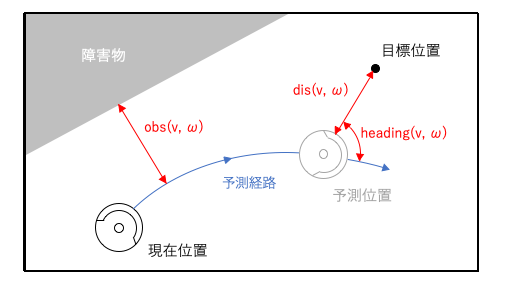
\includegraphics[width=8.5cm]{./picture/DWA.png}
	\caption{局所経路計画における評価}
	\label{fig:DWA}
\end{figure}

\subsection{白線検知}
白線検知にはオープンソースソフトウェアのOpenCV\cite{opencv}を用いて作成した.WEBCAMから取得したRBG画像を,グレー化,ぼかし,二値化,境界線の取得,面積によるフィルタリング,形状判断を行い,白線を検出した.以下に詳しく記述する.

まず,WEBCAMからRBG画像を取得し,Eq.\ref{eq:gray}を用いてグレースケール画像を作成した.
\begin{equation}
	gray = Red * 0.299 +  Green * 0.587 + Blue * 0.114
	\label{eq:gray}
\end{equation}
そのグレースケール画像に対してガウシアンフィルタをかけ,二値化の際に画像が煩雑にならないようにした.また二値化では白線のみに反応するように,160を閾値として二値化した.今回の手法では黒い背景に白い物体がある想定で物体の輪郭を検出した.その後,その物体の輪郭から画像上の面積を取得して,大きすぎるものと小さすぎるものは除く処理を行った.また,画像の上半分は白線があると想定される床以外移すことが多いため,上半分にある輪郭は除く処理を行った.最後に,取得した輪郭を矩形で囲み,輪郭の面積$S_{contours}$と矩形の面積$S_{rectangle}$がEq.\ref{eq:kukei}を満たすものだけに絞ることで四角形の判断を行い,白線を検出した.
\begin{equation}
	S_{contours} > S_{rectangle} * 0.8
	\label{eq:kukei}
\end{equation}


\begin{thebibliography}{99}\scriptsize
	\bibitem{ns} http://wiki.ros.org/navigation
	\bibitem{roomba} https://www.irobot-jp.com
	\bibitem{lrf} https://www.hokuyo-aut.co.jp/search/single.php?serial=21
	\bibitem{raspi} https://www.raspberrypi.org/products/raspberry-pi-3-model-b-plus/
	\bibitem{webcam} https://www.logicool.co.jp/ja-jp/product/hd-webcam-c270
	\bibitem{localization} Sebastian Thrun , Wolfram Burgard , and Dieter Fox 著,上田隆	一 訳,確率ロボティクス, 2007
	\bibitem{opencv} https://opencv.org
\end{thebibliography}

\end{document}
